\section{UNIDAD II}
\subsection{Diseño de sistemas de control en espacios de estado}

De manera general un sistema de control se define
\begin{figure}[h!]
    \centering
        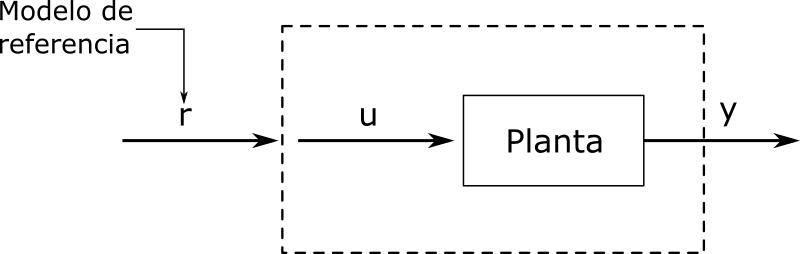
\includegraphics[scale=0.25]{Control de Sistemas Mecatronicos Figuras/03 Sistema de Control.png}
        \caption{Sistema de control}
\end{figure}

donde \( u: \) señal de control, \( y: \) señal disponible. Se asume que la referencia y la salida son conocidas.

En función de \( r \) se definen los siguientes problemas de control:

\begin{enumerate}

    \item Regulación: se considera que \( r \) es constante
        \begin{figure}[h!]
            \centering
                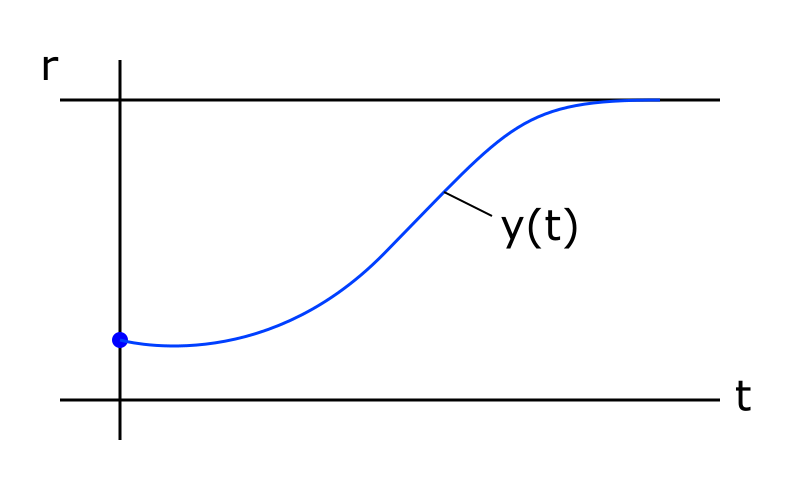
\includegraphics[scale=0.25]{Control de Sistemas Mecatronicos Figuras/04 Regulacion.png}
            \caption{Sistema de control}
        \end{figure}
        
    \item Seguimiento de trayectoria: En este caso \( y \) es una función variante con el tiempo
        \begin{figure}[h!]
            \centering
                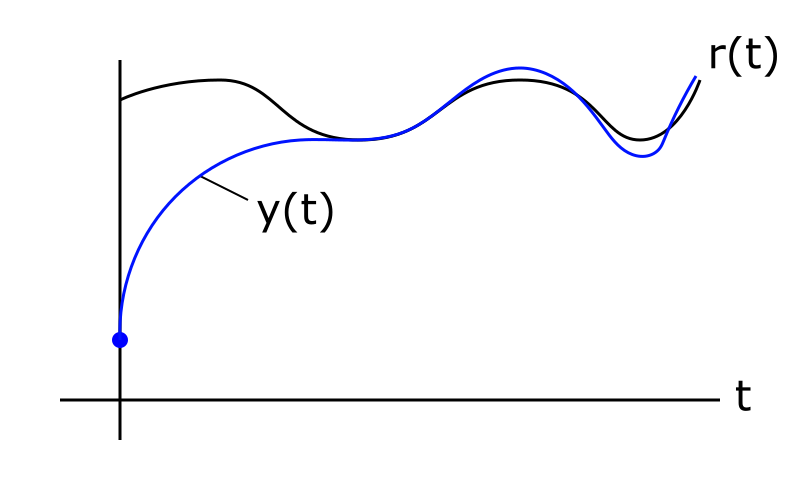
\includegraphics[scale=0.25]{Control de Sistemas Mecatronicos Figuras/05 Seguimiento de Trayectoria.png}
            \caption{Sistema de control}
        \end{figure}
        
    \item Seguimiento de modelo de referencia (Control inteligente)
\end{enumerate}

Los sistemas de control se clasifican en dos tipos principales
\begin{enumerate}

    \item En lazo abierto \\
        \begin{figure}[h!]
            \centering
                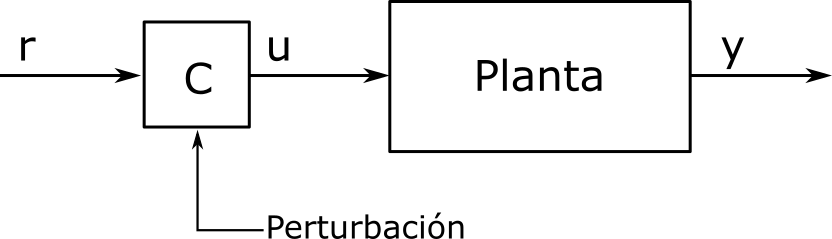
\includegraphics[scale=0.25]{Control de Sistemas Mecatronicos Figuras/06 Lazo Abierto.png}
            \caption{Sistema de control}
        \end{figure}
    La señal de control es independiente de la salida.
    
    \item En lazo cerrado o retroalimentado
        \begin{figure}[h!]
            \centering
                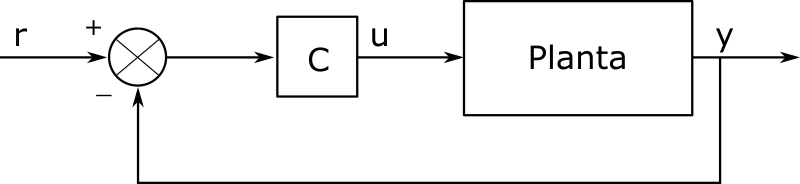
\includegraphics[scale=0.25]{Control de Sistemas Mecatronicos Figuras/07 Lazo Cerrado.png}
            \caption{Sistema de control}
        \end{figure}
\end{enumerate}